% !TeX encoding = UTF-8
% !TeX spellcheck = en_US

\documentclass[
	paper=A4,
	parskip=full,
	chapterprefix=true,
	11pt,
	headings=normal,
	bibliography=totoc,
	listof=totoc,
	titlepage=on,
]{scrreprt}

\usepackage{../../lieb}

\usepackage{feynmp}
\DeclareGraphicsRule{.1}{mps}{*}{}
\graphicspath {{../images/}}

\usepackage{isotope}

\heads{RWTH Aachen \\ Particlephyics Lab}{T8 \\ Positron Lifetime in Matter}{Lieb | Stettner \\ \today} 
\date{\today}

\newcommand{\thirdwidth}{0.32\textwidth}
\newcommand{\halfwidth}{0.48\textwidth}
\newcommand{\fullwidth}{1.0\textwidth}

\setlength\parindent{0pt}
\setlength{\parskip}\medskipamount

\title{Particle Physics Laboratory Class \\ \quad \\ Experiment T8 | Positron Lifetime in Matter}
\author{Jonas Lieb (312136) \\ Jöran Stettner (312169) \\ \\  RWTH Aachen}



\begin{document}

\maketitle

\cleardoublepage

\setcounter{tocdepth}{2}
\tableofcontents

\cleardoublepage

\chapter{Introduction and Theory}

In this laboratory report, a measurement of the positron lifetime in different materials is presented. The experiment uses the special properties of the positron source: Subsequent to the $\beta^+$-decay of $\isotope[22]{Na}$, the decay product $\isotope[22]{Ne}$ emits a high energy photon which can be used as start signal of the time-measurement. 

\section{Positrons in Matter}
The positron as elementary particle is stable in vacuum but behaves different in matter. It can interact electromagnetically and finally annihilate with an electron to photons. \\
At first, the incoming positrons interact with the electrons of the material and are slowed down. The stopping process can be described by the Bethe-Bloch equation and yields in total to the following time values:

\begin{table}[htbp]
	\centering
	\begin{tabular}{ 
			l
			l
			}
		\toprule
		{Material} & {Stopping Time [$\si{\pico\second}$]} \\ 
		\midrule
		Polyethylen & $\approx 300.22 $ \\
		Aluminum &  $\approx 3.11 $ \\
		\bottomrule
	\end{tabular}
	\caption{Time-values for the stopping of a $\SI{180}{\kilo\electronvolt}$ positron, values from \cite{Lab_manual_T8}. Dominating is the time to slow down to thermal energies $E\approx \SI{0.025}{\electronvolt}$.}
	\label{tbl:stop_times}
\end{table}

\subsection{Positrons in Metals}
Depending on the properties of the surrounding material, it is also possible for a positron to form a bound state with an electron, the so called positronium. The conditions can be understood in the Oere-gap model and show that positrons in metal do not form bound states (too large electron-density)\cite{Lab_manual_T8}. In metals, the lifetime of an incoming positron is therefore expected in the $\si{\pico\second}$ regime.

\subsection{Positrons in Plastic and the Decay of Positronium}

In polyethylen on the other hand, the formation of positronium is possible. This bound state exists in two spin configurations: A singlet state (electron and positron spin add up to zero) and a triplet state (spin-sum equals 1). The decay of the two positronium states differ, see figure \ref{fig:feynman_positronium}. Since these electromagnetic processes conserve Parity, the singlet state has to decay to an even number of photons and the triplet state to an odd number\cite{Lab_manual_T8}. \\
Furthermore, the conversion between the two positronium states is possible in matter (e.g. exchange of the electron). This process is more likely and therefore faster than the decay of the triplet state. Concluding, in plastic the formation of positronium is expected which subsequently decays to two photons either directly (singlet state, short lifetime)  or after a conversion (triplet state, longer lifetime/conversion time).

\begin{figure}
	\centering
	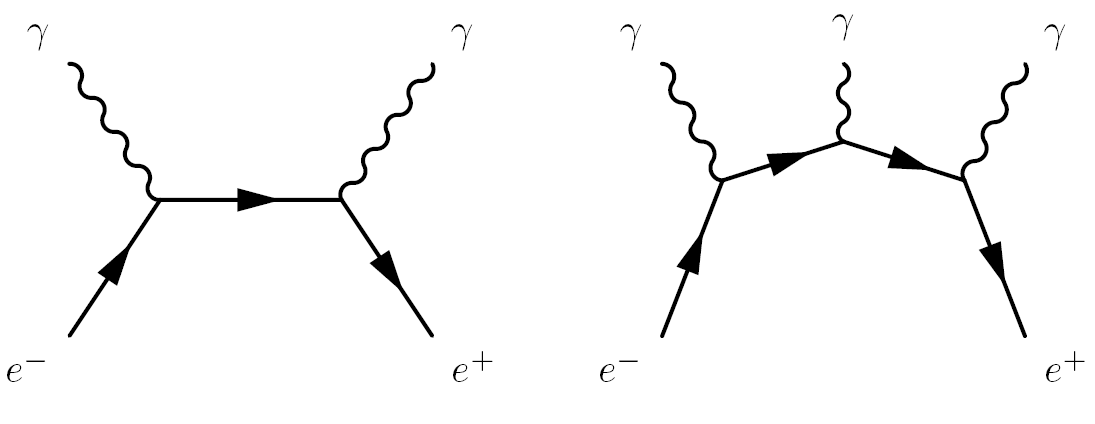
\includegraphics{feynman_positroniumdecay} \\
	\caption{Feynman Diagrams of the Annihilation processes of a positron with an electron (from the surrounding material of from the bound state in positronium),taken from \cite{Lab_manual_T8}. In presence of a nucleus which absorbs an outgoing photon, the annihilation to one photon is possible as well (supressed).}
	\label{fig:feynman_positronium}
\end{figure}


\chapter{Experimental Setup}

The measurement of the lifetime is based on the property of the positron source $\isotope[22]{Na}$ which emits nearly instantaneously a photon in the subsequent decay ($\isotope[22]{Ne}^*\rightarrow \isotope[22]{Ne} $). The idea is to use this gamma ray with an energy of $E = \SI{1.2}{\mega\electronvolt}$ as start signal for the time measuremnt and one of the photons from the positron annihilation as stop signal ($E=\SI{511}{\kilo\electronvolt}$). The high energy photons are detected with plastic scintillators where they mostly create a high energy compton electron which subsequently produces scintillation light. Next to the scintillators on each side of the sample, two photomultiplier tubes (PMTs) are installed where the scintillation photons are converted to an electrical signal. The PMTs provide two signals: One at the last dynode and finally an integrated signal from the anode. The detector setup is schematically shown in figure \ref{fig:positron_setup}.

\begin{figure}
	\centering
	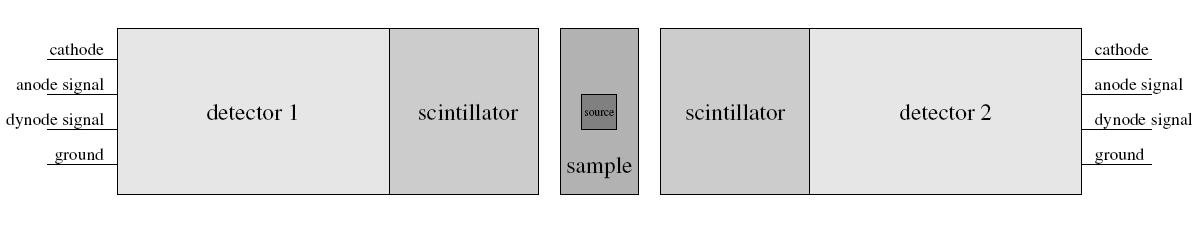
\includegraphics{positron_setup}
	\caption{Scheme of the experimental setup, taken from \cite{Lab_manual_T8}.}
	\label{fig:positron_setup}
\end{figure}

The two signals from each PMT are processed in a coincidence circuit which consists of different modules to reject background. The full electrical circuit is shown in figure \ref{fig:XXX}. The processing of the anode signal consists of the following steps: To reject background, the signal height is compared to a threshold in a Constant Fraction Discriminator (CFD) which provides a NIM-pulse and prevents 'time walk'\cite{Lab_manual_T8}. The actual measurement of the time difference between the start and the stop photons takes place in the Time Amplitude Converter (TAC) which charges a capacitor for the time between the two signals and delivers a pulse after discharging over a resistor. The pulse height is analyzed in a Multi Channel Analyzer module (MCA) and filled in a histogram. Parallel to this, the signals from the last dynode are processed and used to tune the setup for the photons of interest: The dynode signal is proportional to the energy of the initial photon and can thus be used to reject events where the energy does not match the expectation. The signal processing after the two PMTs is therefore specialized: One circuit accepts signals as expected from the first initial photon ($\gamma$ from \isotope[22]{Ne}) and the other from the annihilation photons ($e^+e^- \rightarrow 2\gamma$). The adjustment of these energy windows which are accepted is described in section \ref{sec:PrepandCal}. If both dynode signals pass the Window Discrimators (WD), they are used as coincidence signal and trigger the gate of the MCA. Only in this case, the pulse from the TAC is filled in the histogram. 

\chapter{Preparation and Calibration of the Circuit}
\section{Adjustment of the Window Discriminators}
\section{Adjustment of the Constant Fraction Discriminators}
\section{Synchronization of the Gate and the TAC Signal}
\section{Time Calibration and Determination of the Electronical Resolution}

\chapter{Conduction and Analysis}

\chapter{Systematic Uncertainties}

\chapter{Results and Conclusion}


\cleardoublepage

\bibliographystyle{utphys}
\bibliography{T8_bib}{}

\end{document}


